% !TeX root = ../main.tex

% why not Sport M1 dataset
% why we used crops
% why we used which input-output length
% why we used movement-detection (any describe how)
% how we define an epoch for each
% dataset details (overview as a table?)
% why we used these datasets

% UCF / PAC: show patches AND full-images seq. examples :)



\chapter{Datasets} \label{chapter:datasets}

This chapter presents all datasets that are going to be used in the following evaluation. We have chosen three different video datasets that have been used in related works in order to be able to compare the results and analyze the strength and weaknesses of the different network models. The selected datasets will be introduced one after another ordered by their content's complexitiy with respect to the possible variations in colors, motion and pysical environment. Additionally, random samples from each dataset will be shown to get a better idea of how the data that is fed to the network looks like.


\section{Moving MNIST}


We first train our model on a synthetic dataset of black and white images with flying handwritten digits. The \textit{Moving MNIST} was firstly introduced in \parencite{unsup_learn_lstm} and applied in context of video frame prediction. Since then, it was used several times in different follow-up works, such as \parencite{spat_temp_video_autoenc} or \parencite{conv_lstm_nowcasting}. In the proposed setting, each sequence consits of $20$ frame images of size $ 64 \times 64 $ with two random moving digits from the famous MNIST\footnote{MNIST dataset of handwritten digits: \url{http://yann.lecun.com/exdb/mnist/}} dataset in it. 

One major advantage of this simple dataset is that it exhibits a nearly unlimited size, because it can be generated on the fly. When training a model, we therefore randomly choose two random digits from the first $55,000$ digits of the training set and place them on any location of the first image patch. To generate the subsequent frames, we assign a velocity to each digit, whose direction is chosen uniformly from a unit circle. Further, the simple physical rule is applied that the angle of incidence is equal to the angle of reflection when any digit of size $ 28 \times 28 $ touches the wall. Moreover, this enables other interesting properties of the dataset, such as basic dynamics due to having to predict the right trajectory after bouncing off a wall, as well as multiple occlusion effects of overlapping digits. Consequently, even that the generation process of the dataset is that simple, it is hard for a model to generate accurate predictions on the test set without learning a representation that encodes the internal motion within the system \parencite[p. 6]{conv_lstm_nowcasting}. Last but not least, having a simpler dataset at hand allows us to gain a better understanding of the model's behavior in respect to its hyperparameters. Especially in consideration of the very long training time of several days when more complex or even natural videos are used.

\begin{figure}[htpb]
\centering
\begin{subfigure}{1.0\textwidth}
  \centering
  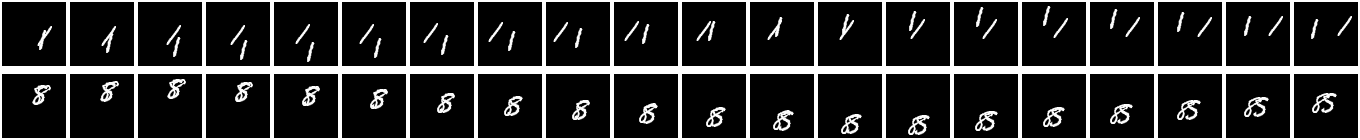
\includegraphics[width=1.0\linewidth]{figures/ds/mm_train.png}
  \caption{Training set}
  \label{fig:mm_train}
  \vspace{.1cm}
\end{subfigure}
\begin{subfigure}{1.0\textwidth}
  \centering
  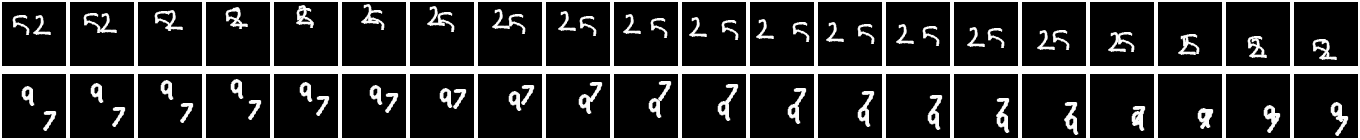
\includegraphics[width=1.0\linewidth]{figures/ds/mm_valid.png}
  \caption{Validation set}
  \label{fig:mm_valid}
  \vspace{.1cm}
\end{subfigure}
\begin{subfigure}{1.0\textwidth}
  \centering
  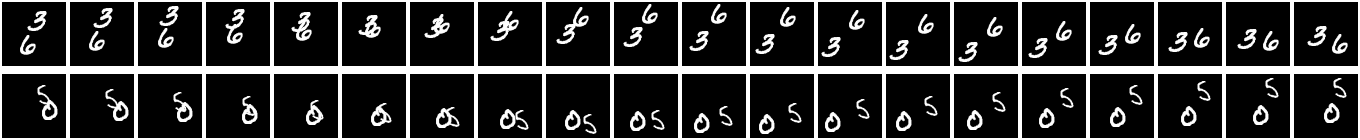
\includegraphics[width=1.0\linewidth]{figures/ds/mm_test.png}
  \caption{Test set}
  \label{fig:mm_test}
\end{subfigure}
\caption[MovingMNIST Image Sequence Samples]{tbd...}
\label{fig:moving_mnist}
\end{figure}

The generation procedure of the validation set is equal to the previously described process to create the training data. But with the difference that the last $5,000$ digits of the original MNIST training split is used. On the contrary, we do not generate the test set on the fly by using the MNIST test split. Instead, we take use of the $10,000$ pre-generate and exaclty $20$ frames long sequences test set used in \parencite{spat_temp_video_autoenc}\footnote{Pre-generated MovingMNIST test set with $10,000$ sequences: \url{http://mi.eng.cam.ac.uk/~vp344/}}. In this way, we are able to achieve more comparable results to at least one competing model. A random sample from each of these splits is presented in Figure \ref{fig:moving_mnist}.

Even that some other works only used a fixed number of pre-generated frame sequences only, we kept up with the on-the-fly generation process of the initial paper for at least three reasons. First, it limits the amound of data and therefore increases the chance of overfitting. Seconds, loading the pre-generated frames from disk takes more time than generating them on the fly; hence it could have a slightly negative impact on the overal performance. And third, it reduces the overall memory requirements in case the whole data would otherwise be pre-loaded into memory in order to eleminate the second mentioned issue.

\subsection*{Characteristics}
\subsection*{Preprocessing}

\section{MsPacman}

Medium complexity, etc
List characteristics (size, splits) and data preprocessing
\subsection*{Characteristics}
\subsection*{Preprocessing}

\begin{figure}[htpb]
\centering
\begin{subfigure}{1.0\textwidth}
  \centering
  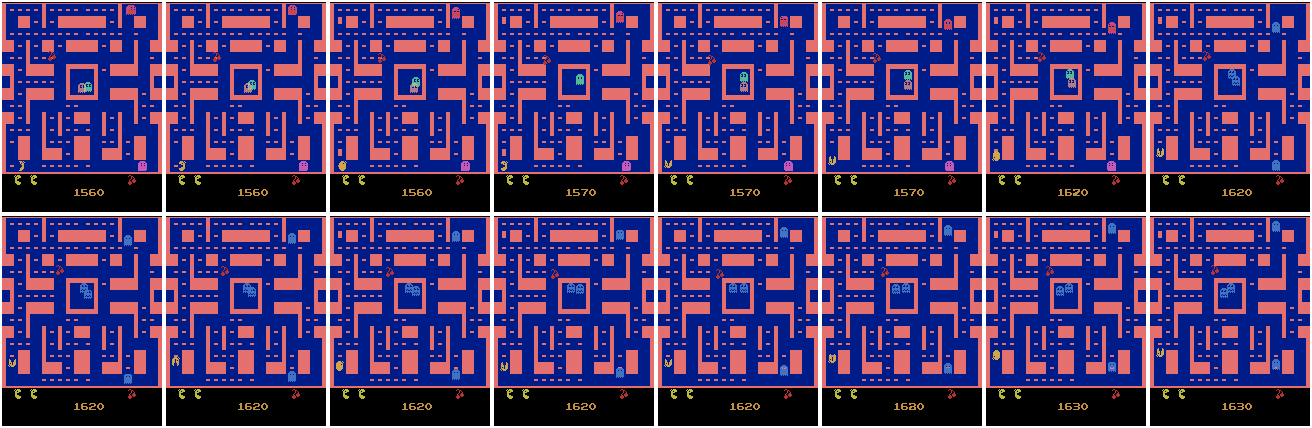
\includegraphics[width=1.0\linewidth]{figures/ds/pac_train_full.png}
  \caption{Training set}
  \label{fig:pac_train_full}
  \vspace{.1cm}
\end{subfigure}
\begin{subfigure}{1.0\textwidth}
  \centering
  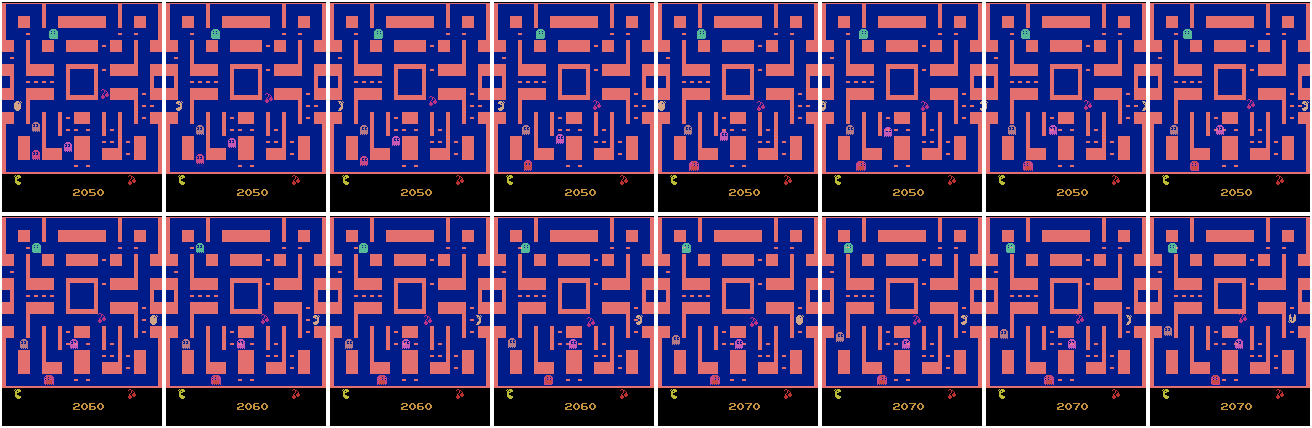
\includegraphics[width=1.0\linewidth]{figures/ds/pac_valid_full.png}
  \caption{Validation set}
  \label{fig:pac_valid_full}
  \vspace{.1cm}
\end{subfigure}
\begin{subfigure}{1.0\textwidth}
  \centering
  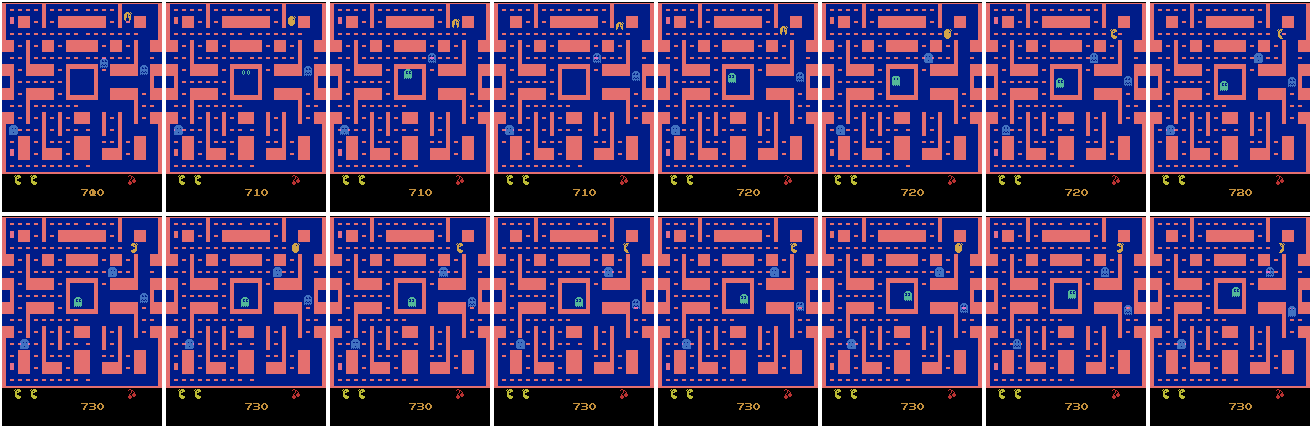
\includegraphics[width=1.0\linewidth]{figures/ds/pac_test_full.png}
  \caption{Test set}
  \label{fig:pac_test_full}
\end{subfigure}
\caption[MsPacman Image Sequence Samples]{tbd...}
\label{fig:pacman_full}
\end{figure}


\begin{figure}[htpb]
\centering
\begin{subfigure}{1.0\textwidth}
  \centering
  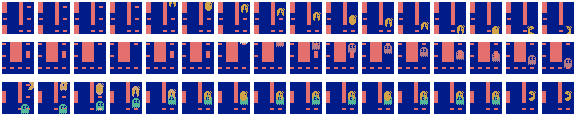
\includegraphics[width=1.0\linewidth]{figures/ds/pac_train.png}
  \caption{Training set}
  \label{fig:pac_train}
  \vspace{.1cm}
\end{subfigure}
\begin{subfigure}{1.0\textwidth}
  \centering
  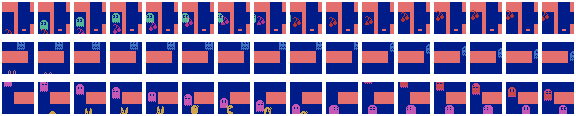
\includegraphics[width=1.0\linewidth]{figures/ds/pac_valid.png}
  \caption{Validation set}
  \label{fig:pac_valid}
  \vspace{.1cm}
\end{subfigure}
\begin{subfigure}{1.0\textwidth}
  \centering
  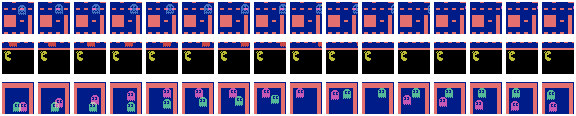
\includegraphics[width=1.0\linewidth]{figures/ds/pac_test.png}
  \caption{Test set}
  \label{fig:pac_test}
\end{subfigure}
\caption[MsPacman Image Sequence Samples]{tbd...}
\label{fig:pacman}
\end{figure}


\section{UCF-101}
% The UCF-101 dataset (soomro et al, 2012) contrains 13,320 videos with an average length of 6.2 sec belonging to 101 different action catergories. The dataset has 3 std. train/test splits with the training set containing around 9,500 videos in each split (the rest are test).
% Sports-1M dataset: (karpathy et al, 2014) contains 1 million youtube clips. even it is labled for actions, we did not do any supervised experiments on it because of logisical constraints with working with such a huge dataset. We instead collected 300h of video by randomly sampling 10 second clips from the dataset.
% we extracted videos where a lot of motion is happening and where there are no shot boundries.
% LSTM-Unsup-paper: "however, we did not do so (movement filter) with Sport1-M, in the spirit of unsupervised learning, and because we did not want to introduce any unnatural bias in the samples."
%   -> we also used UCF-101 for unsupervised training. However, we found that using them did not give any significant advantages over justusing YouTube videos.

% samples at 30 FPS

% Experiments on natural image patches (UCF): Next, we trained to see if our models can also work with natural image pathces. For this, we trainied the models on sequences of 32x32 natural image patches extracted from the UCF-101 dataset. In this case, we used linear output units and the sq-error loss func. The input was 16 frames, ... and predict 13 frames. We

% picutures of other size => crop or pad (ref to fig b)

Natural videos, originally used for action recognition
List characteristics (size, splits) and data preprocessing
\subsection*{Characteristics}
\subsection*{Preprocessing}

\begin{figure}[htpb]
\centering
\begin{subfigure}{1.0\textwidth}
  \centering
  \adjincludegraphics[width=1.0\linewidth,trim={0 {.3333\height} 0 0},clip]{figures/ds/ucf_train_full.png}
  \caption{Training set}
  \label{fig:ucf_train_full}
  \vspace{.1cm}
\end{subfigure}
\begin{subfigure}{1.0\textwidth}
  \centering
  \adjincludegraphics[width=1.0\linewidth,trim={0 0 0 {.3333\height}},clip]{figures/ds/ucf_valid_full.png}
  \caption{Validation set}
  \label{fig:ucf_valid_full}
  \vspace{.1cm}
\end{subfigure}
\begin{subfigure}{1.0\textwidth}
  \centering
  \adjincludegraphics[width=1.0\linewidth,trim={0 0 0 {.3333\height}},clip]{figures/ds/ucf_test_full.png}
  \caption{Test set}
  \label{fig:ucf_test_full}
\end{subfigure}
\caption[UCF-101 Image Sequence Samples]{tbd...}
\label{fig:ucf_full}
\end{figure}


\begin{figure}[htpb]
\centering
\begin{subfigure}{1.0\textwidth}
  \centering
  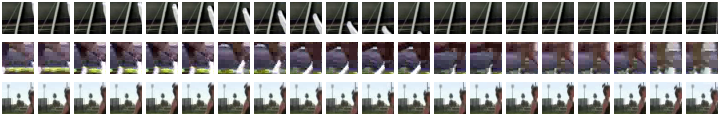
\includegraphics[width=1.0\linewidth]{figures/ds/ucf_train.png}
  \caption{Training set}
  \label{fig:ucf_train}
  \vspace{.1cm}
\end{subfigure}
\begin{subfigure}{1.0\textwidth}
  \centering
  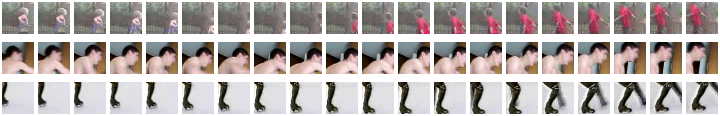
\includegraphics[width=1.0\linewidth]{figures/ds/ucf_valid.png}
  \caption{Validation set}
  \label{fig:ucf_valid}
  \vspace{.1cm}
\end{subfigure}
\begin{subfigure}{1.0\textwidth}
  \centering
  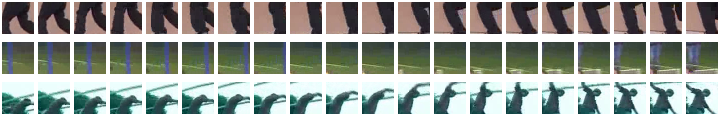
\includegraphics[width=1.0\linewidth]{figures/ds/ucf_test.png}
  \caption{Test set}
  \label{fig:ucf_test}
\end{subfigure}
\caption[UCF-101 Image Sequence Samples]{tbd...}
\label{fig:ucf}
\end{figure}




